%!TEX root = post_review.tex
\section{Complexity}\label{sec:complexity}
We next discuss bounds on the computational complexity of the algorithm outlined in Section~\ref{sec:line:search}.
For a given active set at most $2N$ mpQPs must be solved, and this is done by decomposing the
problem as stated in section~\ref{sec:gen:mpQP}.  For each mpQP the main computational effort is to
determine $\Sigma$ in~\eqref{seq:sigma}. In the case of~\eqref{eq:sigma:normal} this requires a QR
decomposition with $2(mn^2-n^3/3)$ floating point operations (flops, see e.g.~\cite{Golub:1996}), 
where $m$ is the number of active constraints and $n$ the number of
optimisation variables, plus inversion of a triangular matrix with $(m^3-m)/6$ flops and several matrix
multiplications with $mpn$ flops (for the multiplication of a $m\times n$ matrix with a $n\times p$
matrix). The computationally more expensive case of~\eqref{eq:sigma:degen} requires a QR decomposition,
inversion of a definite matrix $W$ using Cholesky decomposition with $n^3/3$ flops, inversion of a triangular
matrix, several matrix multiplications and additions with $mn$ flops, and inversion of a definite matrix
$\Delta$. In the worst case this adds up to at most $11n^3+n^2-n/3$ flops to obtain $\Sigma$. The solution to
the problem is then the result of a matrix multiplication, and, in order to be able to solve the subsequent
mpQP, the matrix $W_\theta$ and the vector $c_\theta$ also need to be computed. Hence the overall flop count
in the worst case adds up to $11n^3+n^2+2/3n+2n^2 n_\theta$, where $n_\theta$ denotes the dimension of the
parameter~$\theta$. 
%At each stage two mpQPs have to be solved recursively, so that 
In the worst case the
recursion for the entire horizon therefore requires $N(2 n_x+5 n_x^2+101 n_x^3+8 n_x^2 (n_u+n_x))$ flops.

The number of active set changes needed to obtain the active set corresponding to the current plant state
is necessarily finite, since this number cannot exceed the total number of possible active sets. However upper
bounds on this number are unrealistically large (except in pathological cases) and hence of little use in bounding the number of times that the recursion of
Section~\ref{sec:line:search} needs to be solved. Instead we give the typical execution time for an example
system with an implementation in MATLAB  in section~\ref{sec:example}.


\section{Example}\label{sec:example}
In this section we present a numerical simulation for a simplified levitating ball model, as derived in~\cite{Schaich:2015}. The dynamics of the nonlinear system are given by $m\ddot y = m g - c i^2/y^2$,
where $m$ denotes the mass of the ball, $g$ is the acceleration due to gravity, $c$ is a constant depending
on the coil, $y$ the vertical distance to the coil (Fig.~\ref{fig:levitating:ball}). We assume that the current~$i$ is directly specified by the controller, thus neglecting the inductive dynamics of the coil. %Figure~\ref{fig:levitating:ball} illustrates the setup.
Choosing the state $x=(y,\dot y)$ and the input $u=i$ we obtain a state space representation which depends nonlinearly
on the state and control input. For any $x_1>0$, the system is in equilibrium if $x_2=0$ and $u=\sqrt{\frac{gm}{c}}x_1$.

Linearising the nonlinear differential 
equation $\dot x = f(x,u)$ around an equilibrium point $(\hat x, \hat
u)$ gives the approximate linear model 
%
\[
	 \Delta\dot{x} = \underbrace{\left(\begin{array}{cc}
	0 & 1 \\ \frac{2c\hat u^2}{m\hat x_1^3} & 0
	\end{array}\right)}_{\frac{\partial f}{\partial x}(\hat x,\hat
      u)}\Delta x 
+ \underbrace{\left(\begin{array}{c}
	0 \\ - \frac{2c\hat u}{m\hat x_1^2}
	\end{array}\right)}_{\frac{\partial f}{\partial u}(\hat x,\hat
      u)}\Delta u
\]
%
where $\Delta u = u -\hat{u}$ and $\Delta x \approx x-\hat{x}$.
We derive the discrete time dynamics with sampling rate $T_s$ using
the Euler formula $x^+=x+T_s f(x,u) =:\tilde f(x,u)$ giving
\[
\Delta x^+ = A \Delta x + B \Delta u , \quad
\Biggl\{\begin{aligned} A &= I+T_s\frac{\partial f}{\partial  x}(\hat
  x,\hat u) \\
B &= T_s \frac{\partial f}{\partial u}(\hat x,\hat u)
\end{aligned}
\]
%
A representation of the form~\eqref{eq:the:problem}, in which the disturbance $w$ accounts for linearisation
errors, can be obtained by sampling input and state
constraints and using the mean-value theorem \citep[see][]{Schaich:2015}. This leads
to a disturbance representation of the form $\mathcal W(x,u)=\{w\in\mathbb R^n: 
\min_{k\in\mathcal S_w}\{ H_{k,i}^x x + H_{k,i}^u u\} \leq w_i \leq \max_{k\in\mathcal S_w} 
\{ H_{k,i}^x x + H_{k,i}^u u \} \}$,
where ${k\in\mathcal S_w}$ denotes the sample index and $i$ the row number. This point-wise polytopic representation
together with a polyhedral representation of state constraints allows us to compute a polyhedral
MRPI set~$\mathcal X^\infty$. As a terminal feedback controller $K$ we use the solution to the robust 
Lyapunov condition $V(x)-V((A+BK)x+Dw)\leq \gamma^2 w^Tw$ 
with $V(x)=x^T P_0 x\geq0$, i.e. $x^TP_0x - ((A+BK)x+Dw)^TP_0((A+BK)x+Dw)\geq x^T(Q+K^TRK)x -\gamma^2 w^T w$, 
\cite[see e.g.][]{Boyd:94}. This semi-definite program can also be used to find the minimum value of $\gamma^2$. Starting from 
a polyhedral MRPI set~$\mathcal X^\infty$ we apply the algorithm presented in section~\ref{sec:preliminaries}
to obtain the necessary stage constraints~$\mathcal Z_k$. At this stage we can introduce numerical values
for individual parameters: $T_s=30\,\text{ms}$, $C=1\,\frac{\text{kg m}^3}{\text{A}^2\text{s}^2}$,
$m=100\,\text{g}$, $\hat x_1 = 50\,\text{mm}$ and $\mathcal X=\{x:
\abs{x_1- \hat x_1}\leq 1\,\text{mm}\wedge \abs{x_2}\leq 105\,\frac{\text{mm}}{\text{s}}\}$, $\mathcal
U=\{u:\abs{ u-\hat u}\leq 10 \,\text{mA}\}$.
To obtain $\mathcal W(x,u)$ we sample $\mathcal X$ and $\mathcal U$ with a total of 25 samples, i.e. the cardinality
of $\mathcal S_w$ is 10. In the simulation we use horizon length $N=5$. We perform a cold started line search from $\chi_0=(0,0)$
to the outer bound of the constraint set at $\chi_e=(1,-30)$, the resulting trajectories at the boundaries of
individual active sets are plotted in Figure~\ref{fig:plot}.

The simulation was implemented in MATLAB using only non-optimised built-in functions for the main computational
purposes. In the simulation illustrated in Fig.~\ref{fig:plot} a total of $10$ iterations were required,
of which $7$ correspond to changes of the dominating right hand side of $\mathcal W(x,u)$, for which no
recomputation of the solution is necessary. For $\chi_e$ on the boundary of the feasible set
the solution time is less than $0.5\, \text{s}$ in total (using a MacBook Pro with a $2.3\,\text{GHz}$ quad-core processor).

\begin{figure}
\centering
% \begin{overpic}[scale=0.75]{levitatingBall}
% \put(30,5){$m g$}
% \put(30,41){$c\frac{i^2}{x^2}$}
% \put(78,28){$y$}
% \put(90,89){$i$}
% \end{overpic}
\begin{lpic}{levitatingBall(.75,)}
\lbl[tr]{25,3; $m g$}
\lbl[br]{25,25; $c\frac{i^2}{y^2}$}
\lbl[bl]{49,17; $y$}
\lbl[bl]{56,55; $i$}
\end{lpic}
\vspace{-2mm}
\caption{Levitating ball system.}
\label{fig:levitating:ball}
\end{figure}

\begin{figure}
\centering
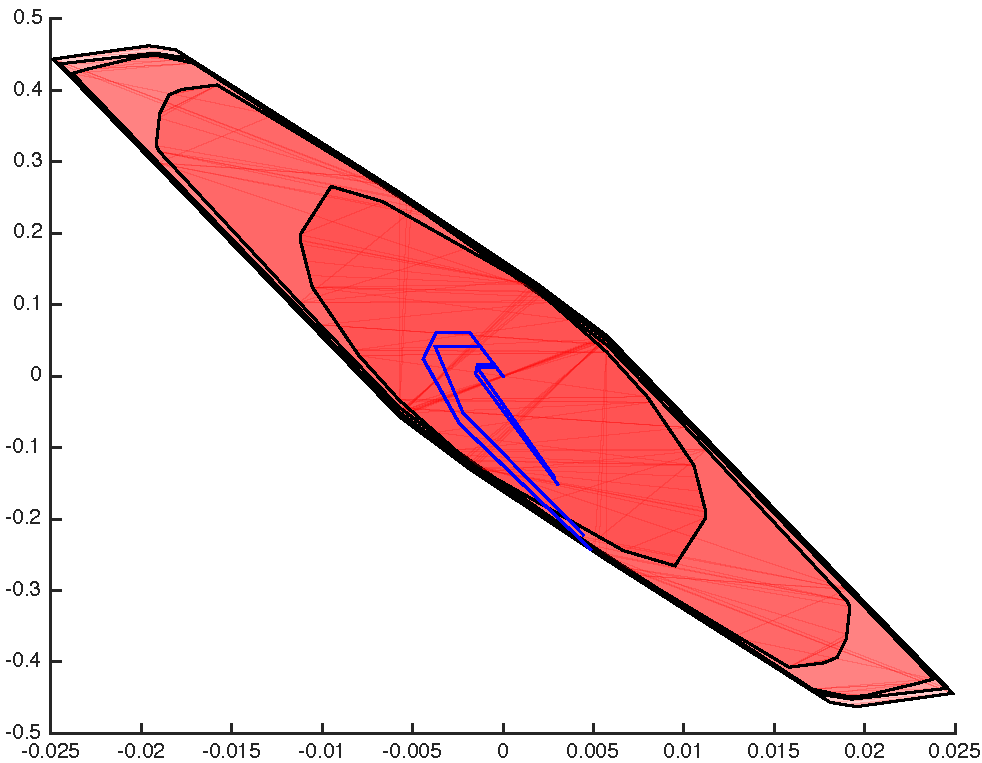
\includegraphics[width=\columnwidth]{myplot}
\caption{Projected stage constraints $\mathcal X_i, i=1,\dots,N$ in red. Trajectories
at the active set changes and on the boundary in blue.}
\label{fig:plot}
\end{figure}

% This section we present a numerical simulation in which the state-dependent uncertainty enters through an upper bound on the linearisation
% error for a nonlinear system. We consider an inverted pendulum described by $ml^2\ddot\varphi = mlg\sin\varphi+M$, where
% $m=0.1$\,kg is the mass, $l=0.3$\,m is the length of the pendulum, $g=9.81$\,m\,s$\mbox{}^{-2}$ is the gravitational
% constant and $M$ is the direct torque input. Discretisation using Euler backward finite differences 
% at $f = 20$\,Hz yields
% \begin{equation}
%   \begin{split}
%     x_1[k+1] &= x_1[k] + \frac{1}{f} x_2[k]\\
%     x_2[k+1] &= \frac{g}{fl} \sin(x_1[k]) + x_2[k] + \frac{1}{fml^2}u[k]
%   \end{split}
% \end{equation}
% where $x_1[k] = \varphi(t_0+k/f),x_2[k] = \dot\varphi(t_0+k/f)$ and $u[k] = M(t_0+k/f)$.
% The nonlinearity is given by the sine function, and we can explicitly state the 
% linearisation error as $e(x_1)=\frac{g}{fl}(\sin x_1 - x_1)$. Since the linearisation
% only approximates the nonlinear dynamics around the equilibrium we can choose a closed interval 
% $0\in D\subset\mathbb R$ and maximise the upper bound 
% \begin{equation}
%   \Delta e = \max_{x_1\in D}\abs{\frac{de}{dx_1}} = \frac{g}{fl}\max_{x_1\in D}\abs{\cos x_1-1}.
% \end{equation}
% This results in the linear system
% \begin{equation}
%   x^+ = \underbrace{\left(\begin{array}{cc}
%   1 & f^{-1}\\ g(fl)^{-1} & 1
%   \end{array}\right)}_A x + \underbrace{\left(\begin{array}{c} 0 \\(ml^2f)^{-1} \end{array}\right)}_B u
%   +\left(\begin{array}{c}w_1\\ w_2\end{array}\right)
% \end{equation}
% with $\abs{w_1}\leq w_{1,\max}$ and $\abs{w_2}\leq\max\{w_{2,\max},\Delta e \abs{x_1}\}$.
% We also introduce the input constraint $\abs{u}\leq3$\,N\,m and use the interval $D = [-\frac{3\pi}{4},
% \frac{3\pi}{4}]$ and a horizon of $N=7$ to obtain the sequence of state constraints $\mathcal X_m$
% depicted in Figure~\ref{fig:numerical:example}. The line search starting at the origin and
% exploring towards $\mathpzc x_e=(-6,50)$ produces the optimal trajectories at the active-set switches
% which are illustrated in blue. In pink a warm-started line search terminates on the boundary of the
% feasible set before reaching the (infeasible) state $\mathpzc x_e=(0,30)$.